\documentclass{article}
\usepackage{color}
\usepackage{listings}
\usepackage{graphicx}
\lstset{ %
language=java,                % choose the language of the code
basicstyle=\footnotesize,       % the size of the fonts that are used for the code
numbers=left,                   % where to put the line-numbers
numberstyle=\footnotesize,      % the size of the fonts that are used for the line-numbers
stepnumber=1,                   % the step between two line-numbers. If it is 1 each line will be numbered
numbersep=5pt,                  % how far the line-numbers are from the code
backgroundcolor=\color{white},  % choose the background color. You must add \usepackage{color}
showspaces=false,               % show spaces adding particular underscores
showstringspaces=false,         % underline spaces within strings
showtabs=false,                 % show tabs within strings adding particular underscores
frame=single,           % adds a frame around the code
tabsize=2,          % sets default tabsize to 2 spaces
captionpos=b,           % sets the caption-position to bottom
breaklines=true,        % sets automatic line breaking
breakatwhitespace=false,    % sets if automatic breaks should only happen at whitespace
escapeinside={\%*}{*)}          % if you want to add a comment within your code
}
\begin{document}
\tableofcontents{}


\newpage
\section{Einführung}
Performanz spielt eine große Rolle in der Entwicklung von Software und Hardware.
In meiner Arbeit werde ich mit dem fio Tool arbeiten, um solche Performanzänderungen zu berechnen und zu analysieren.
Fio ist ein Programm mit der man die Hardware-Performanz testen kann, z.B die Brandweite beim Schreiben einer Datei, und die Performanz als log Daten ausgeben kann.
Mein Programm wird mit diesen Logs arbeiten, um sie besser darzustellen und arbeiten zu können. Ziel meines Tools soll es sein, dass man den stationären Zustand analysiert.


\section{Grundlagen}
Mit dem fio (flexible Input/Output) Programm, kann man die Performanz auf einer bestimmten Hardware testen .
fio besitzt kein GUI sondern arbeitet nur in der Konsole. Man kann für das Programm fio-Dateien schreiben oder auch in der Konsole arbeiten, um seine gewünschten Task zu testen,
wie random read/write auf einer Datei.
Wenn man ein Random Read testen möchte, kann die fio-Datei so aussehen.

\begin{lstlisting}
    ; fio-rand-read.job for fiotest

    [global]
    name=rand-read # Name des Jobs
    rw=randread # Was soll der Job testen, randread = random read
    runtime=2s # Wie lange soll der Job laufen
    size=2m # Groesse der Datei, m fuer Megabyte
    write_bw_log=mytest # Name der Log-Datei

\end{lstlisting}
In der Konsole gebt man sie als Parameter an, wenn es nur ein schneller Test sein soll. Zusätzlich können die Tests, 
oder auch Jobs genannt, Logs ausgeben. Mit diesen Logs wird mein Tool arbeiten. Dieser Job oben testet das Random-Read mit einer
runtime von 2 Sekunden. Nun möchte man wissen wann der stationäre Zustand erreicht wurde, wenn man solche Tests länger durchlaufen lässt.
Der stationäre Zustand ist der erreichte Zeitpunkt, wenn es keine starken Schwankungen mehr bei der Brandweite im Lesen und Schreiben gibt.
Das Schreiben und Lesen verhält sich außerdem nicht deterministisch. Das bedeutet, auch wenn man die selbe Datei mit dem Selben Computer lesen/schreiben
würde, wäre die Brandweitengeschwindigkeit immer im Durchschnitt unterschiedlich.

\section{Konzept}
Mein Tool soll mit den Logs von fio arbeiten. \newline
Mit dem Parameter $write\_bw\_logs=[Dateiname]$, kriege ich eine Datei mit jeweils 5 Spalten:
\begin{lstlisting}
    Time,	Bandwidth,	data direction, Blocksize,	Offset
    0, 	    59782, 		0,		        4096,		0
\end{lstlisting}
Time für die Zeit in Millisekunden (ms) die verlaufen ist, Bandwidth für die Brandweite in Megabyte/ms
für das random read, Date direction ob gelesen (= 0) oder geschrieben (= 1) wurde
und ein Offset. Die Log Daten sind immens Lang und nicht schön lesbar. Deshalb wurde schon ein Tool in Python gebaut 
was diese log Daten auswertet. Für Veranschaulichung habe die das fio Programm auf meinem Rechner laufen lassen mit dem
Command die oben erwähnt wurde. Die log Datei wurde ausgewertet und als .svg Datei ausgegeben:
\begin{figure}[ht!]
    \centering
    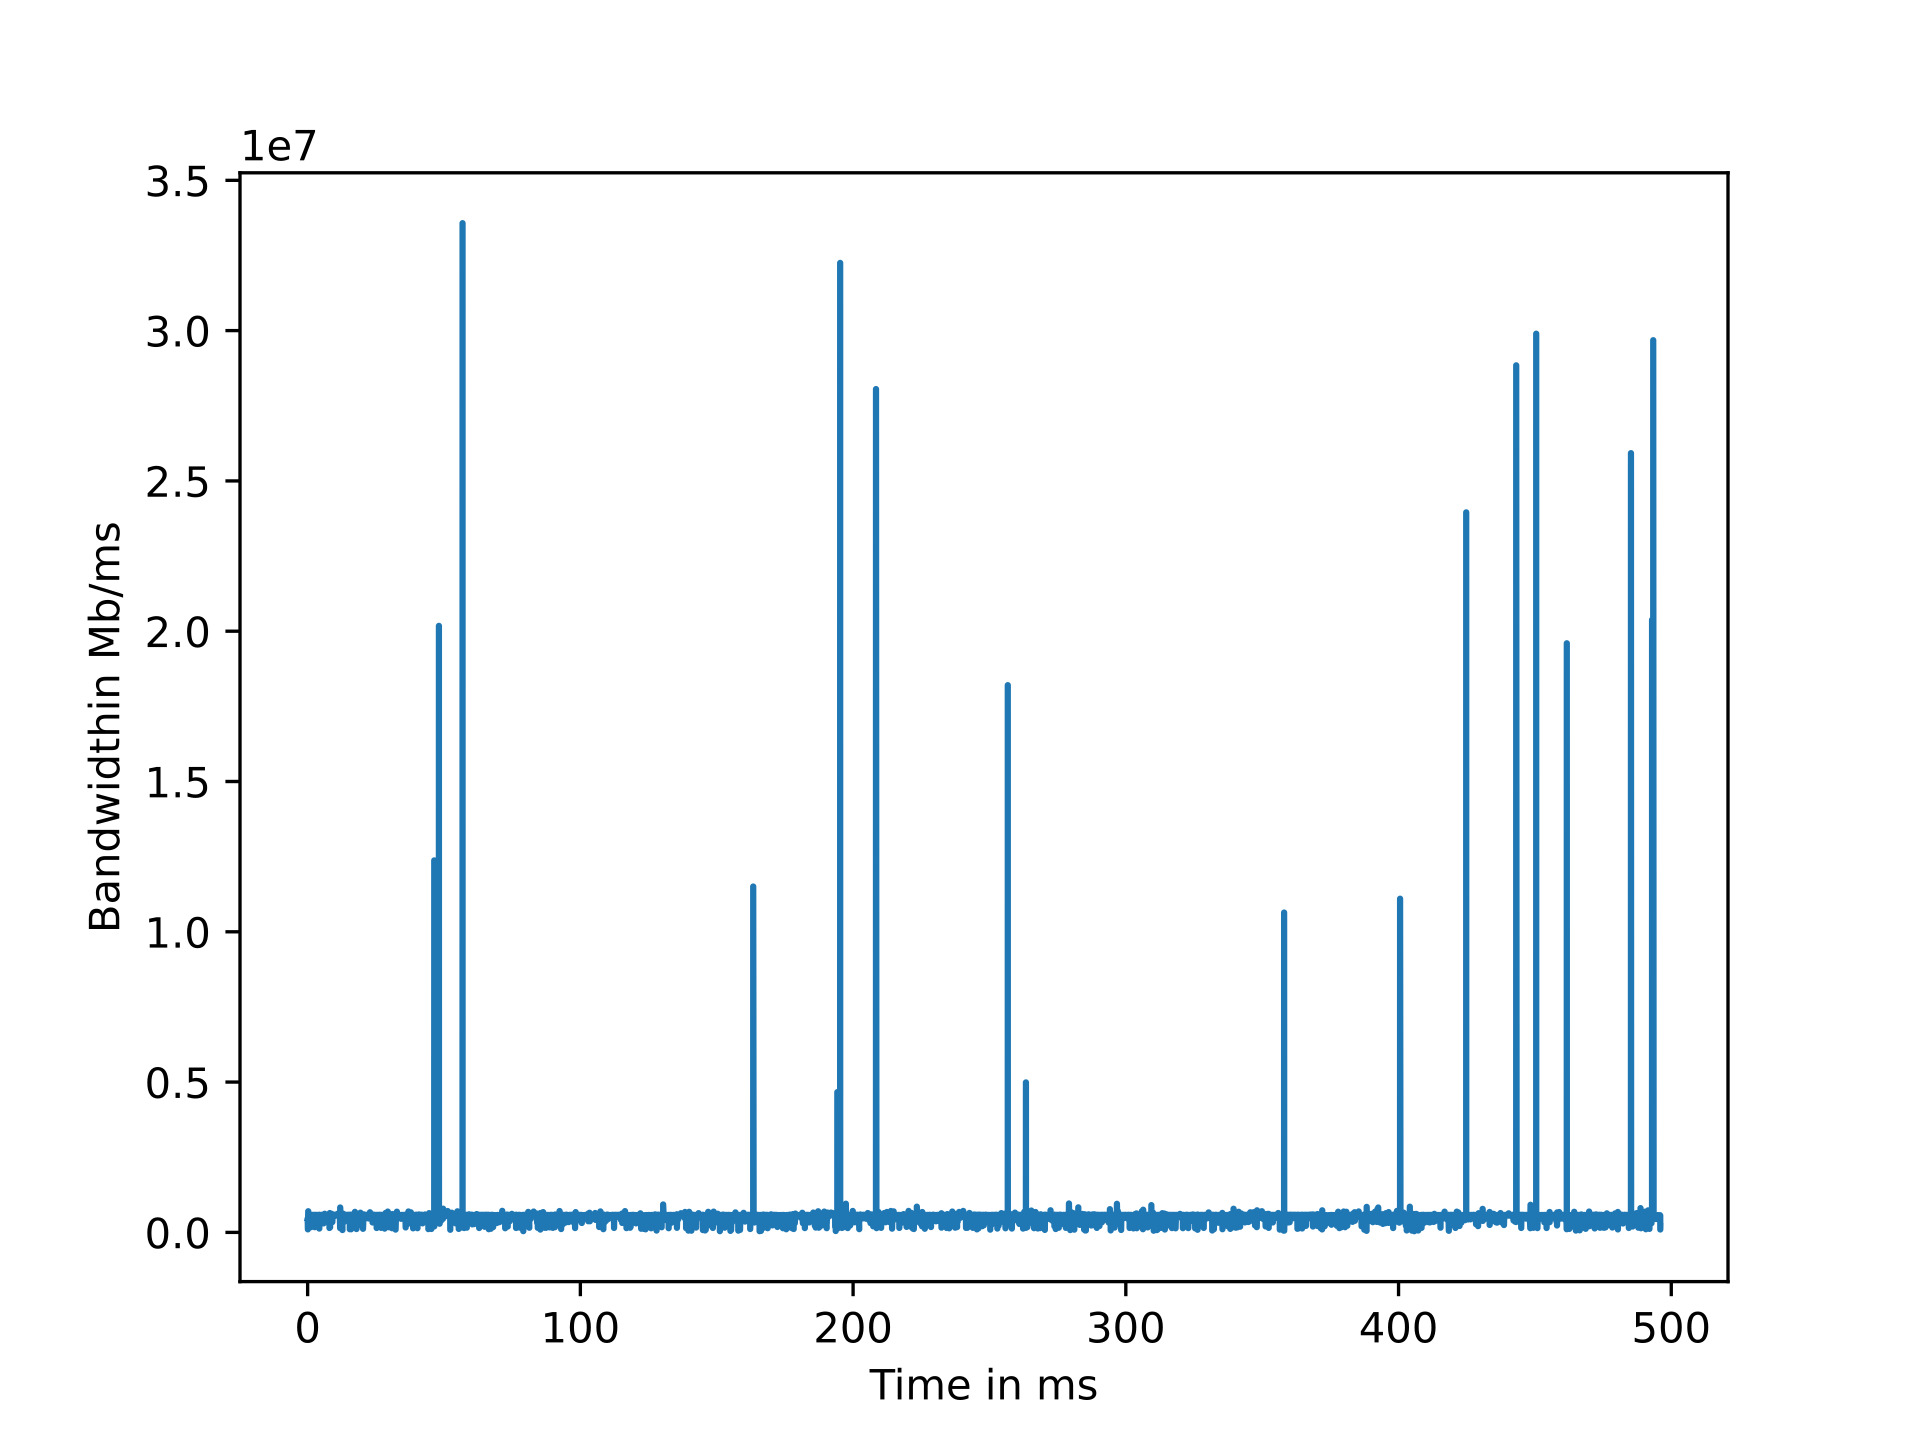
\includegraphics[width=120mm]{./Code/nm_mytest_bw.jpg}
    \caption{Plot tool Ausgabe mit Log Datei  \label{overflow}}
    \end{figure}

\section{Verwandte Arbeiten}
\section{Zeitplan}
\end{document}